\documentclass[10pt]{standalone}
\input{../../tikzpic_packages.tex}

\def\pneumaticcolor{blue!20}

\begin{document}
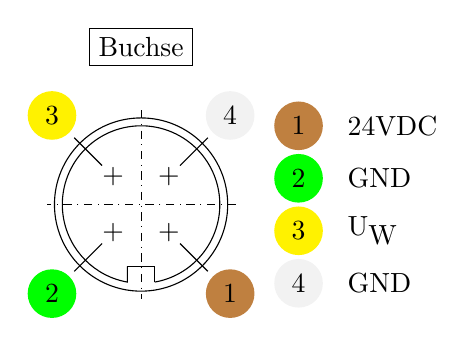
\begin{tikzpicture}[
]

\path (0,2) node[draw]{Buchse};

\def\dangle{10}
\draw (0,0)++(-90+\dangle:1)coordinate(X)arc(-90+\dangle:270-\dangle:1)--++(0,.2)coordinate(XX);
\draw (X)--++(0,.2)--(XX);
\draw (0,0)circle (1.1);

\draw[dashdotted] (1.2,0)--(-1.2,0) (0,1.2)--(0,-1.2);


\foreach[count = \i] \angle/\col/\t in {315/brown/24VDC,225/green/GND,135/yellow/U$_\textnormal{W}$,45/gray!10/GND}{
	\draw (\angle:0.5)node{+}++(\angle:.2)--++(\angle:.5)++(\angle:.4)node[circle,fill=\col]{\i};
	\pgfmathsetmacro{\y}{(\i-1)/3*2}
	\path (2,1-\y)node[circle,fill=\col]{\i}++(.5,0)node[right]{\t};
}

\end{tikzpicture}
\end{document}